\documentclass[11pt]{article} % 11pt font
\usepackage{amsmath}
\usepackage{amsfonts}
\usepackage{bm}
\usepackage{graphicx}
\usepackage{mathtools}
\usepackage{physics}
\usepackage{pgfplots}
\usepackage{accents}
\usepackage{geometry}
\usepackage{tikz}
\usepackage{caption}
\usetikzlibrary{quantikz2}

% my custom commands
% ------------------
% note command
\newcommand{\note}[1]{\textsf{\textcolor{red}{#1}}}
% multi-line comment command
\newcommand{\comment}[1]{}
\newcommand{\unit}{1\!\!1}
\graphicspath{{./images}}


% -------------------------
% BEGINNING OF THE DOCUMENT
% -------------------------
\begin{document}

\section{Overview}
Quantum Computers are slower overall but with better asymptotic complexity. \\
There are many kinds of quantum computers (Superconducting, vacancy center, trapped ion, photonic). \\
Peter Shor showed that you can factorize large products of primes can be computed faster on a quantum computer. \\
IBM was one of the first companies to try and build a quantum computer. \\
\subsection{Why Quantum Computers}
Why is a quantum computer more powerful? We look at the space we need to describe such a system:\\
For a system of 3 spins we can see
\begin{align*}
	\ket{\psi_1} &= \alpha\ket{\uparrow_1} + \beta\ket{\downarrow_1} \\
	\ket{\psi} &= \alpha_1\ket{\uparrow\uparrow\uparrow} + \alpha_2\ket{\uparrow\uparrow\downarrow} + \ldots
\end{align*}
We can see that in order to represent $N$ terms, we need $2^N$ complex coefficients. The Hamiltonian needs $2^{2N}$ coefficients to represent the systems evolution. \\
Measurement only gives us $N$ bits of information on the output, therefore we kinda lose our advantage :(
\section{Classical Computing}
\subsection{Computation as a physical process}
All information used by a classical computer is stored as a sequence of zeroes and ones. These two must be physically different. In a classical computer we typically store a zero by a low voltage, and a 1 by a high voltage (these voltages should be quite different). This can done by switching between $100 \Sigma$ and $10k\Sigma$ resistances. \\
For a single bit we can construct four distinct gates. Of these two of these are reservable and two are irreversible. These gates can be represented by truth tables.\\
A reversible gate may be the not gate.
\begin{displaymath}
\begin{array}{| c | c |}
	\text{in} & \text{out} \\
	\hline
	0 & 1 \\
	1 & 0
\end{array}
\end{displaymath}
An irreversible gate may be a zero gate:
\begin{displaymath}
\begin{array}{| c | c |}
	\text{in} & \text{out} \\
	\hline
	0 & 0 \\
	1 & 0
\end{array}
\end{displaymath}
This is thermodynamically irreversible as the zero gate lowers the entropy. Since entropy should increase then in order to do this operation we must produce heat elsewhere.
\begin{align*}
	\Delta Q &= k_B T\ln Z
\end{align*}
We also generate heat since we don't make any transformations adiabatically, since adiabatic transformations would be much slower. \\
Moving on to two-bit gates. We first look at:
\begin{displaymath}
\begin{array}{| c c | c c |}
	\text{input 1} & \text{input 2} & \text{out 1} & \text{out 2} \\
	\hline
	0 & 0 & 0 & 0\\
	0 & 1 & 0 & 1\\
	1 & 0 & 1 & 1\\
	1 & 1 & 1 & 0
\end{array}
\end{displaymath}
How many 2-bit gates are there? \\
There are $256$ total gates ($4^4$) and then $24$ reversible gates  ($4!$ aka the number of permutations of the gates). Product operations make up $16$ total states and $4$ reversible states. Any computation can be constructed from single bit and controlled not gates. \\
You can do classical computations reversibly? This can be done by storing some of the input as the output, i.e. $2 \cross 5 = 10,2$. For generalized computation we will need all the reversible single bit gates and the controlled controlled not. \\
In a quantum computer all gates must be reversible. On a quantum computer you only need single bit gates, controlled nots and measurements.
\subsection{Complexity classes}
A complexity class determines the scaling of an algorithm as the input asymptotically increases. This is typically thought of in terms of the average, or worst case complexity. We don't include any prefactors here. \\
Example: schoolyard multiplication scales as $O(n^2)$ \\
Simulating a quantum system grows exponentially. \\
Example: For a database with n elements, sorting the database can be done using the simple swapping method. For an upper bound we can say it takes $n^2$ assuming that we do a sort of insertion sort. For a lower bound we assume the list is already sorted, so the complexity must be between $O(n^2)$ and $O(n)$

`
\subsection{Complexity Classes continued}
How Computer Scientists classify how to solve problems.\\
We first define the class of efficiently solvable problems as $P$, such that the problems emit solutions that are bounded above by some polynomial function $S(n)$. \\
Even though this could include algorithms with horrible scaling properties this can be typically solved much quicker. \\
The next set of complexities is $N-P$, which emits solutions that can be verified in a polynomial number of steps. \\
Whether or not there is a difference between $P$ and $N-P$ is an unsolved problem (though intuitively they should be different). \\
Inside NP there is a set of problems known as $N-Pc$ or $NP$ complete, which map to all other $N-P$ problems in polynomial time, i.e. if any $N-Pc$ problem was solved in polynomial time, then all $N-P$ problems can be solved in polynomial time. \\
The SAT problem is inside $N-Pc$. This problem requires satisfying a set of boolean statements by choosing the correct set of input values. Clearly this can map to any problem in some polynomial time. \\
3-SAT is also in $N-Pc$ but the boolean statements only contain at most 3 variables in each equation. \\
2-SAT is instead in $P$. \\
Traveling salesman is in $N-Pc$. \\
We now introduce a new complexity set, this is $BQP$, bounded error probability quantum polynomial, which takes polynomial time to solve on a quantum computer with a bounded error probability. \\
We typically have error probabilities less than $30\%$, which means we may need to run the algorithm multiple times to get the correct answer. \\
This includes things like the discrete log problem and factoring. \\
Simulating a quantum system cannot be verified efficiently on a classical computer so any quantum system can be in $BQP$ but not in $NP$. \\
\section{Quantum Computing}
When moving to quantum computing we replace our binary $0$ and $1$ with quantum states $\ket{0}$ and $\ket{1}$, as our basis. We call these qubits. \\
All quantum process have linear time evolution, and as a result any gate must be represented by a linear operator. Additionally conservation of probability (assuming we can't lose our qubit) requires all gates to be unitary.


\subsection{Introduction to Hilbert Spaces}
A vector space $V$, will be defined as normal, with addition, scalar multiplication, inverses and the identity.\\
We add an inner product with the following properties:
\begin{align*}
	(v,w) &\in \mathbb{C} &
	(v,w) &= (w,v)^* \\
	(v.v) &\geq 0 &
	(v,v) = 0 &\leftrightarrow v = 0
\end{align*}
In quantum mechanics we work inside Hilbert Space $H$, which is a completed complex inner product space. We write these vectors in bra-ket notation $\ket{v}$. We choose the standard basis of $\ket{0}$ and $\ket{1}$. We write our inner products in terms of bra-ket notation as well (this corresponds to vectors and covectors in actuality) $(v,w) = \bra{v}\ket{w}$. \\
These vectors in Hilbert space represent the state of a particle. If two vectors are orthogonal, then the two states are distinguishable states. If we have an overall phase shift to our state $\ket{\psi} \to e^{i\phi}\ket{\psi}$ then there is no measurable change to our system. We restrict ourselves additionally to vectors of unit length, because there's no physical impact of large vectors. There are multiple ways to construct things that are analogous to the classical not gate:
\begin{displaymath}
\begin{array}{|c | c|}
	\text{in} & \text{Not} \\
	\hline
	\ket{0} & \ket{1} \\
	\ket{1} & \ket{0}
\end{array}
\end{displaymath}
\begin{displaymath}
\begin{array}{|c | c|}
	\text{in} & \text{Not'} \\
	\hline
	\ket{0} & -\ket{1} \\
	\ket{1} & \ket{0}
\end{array}
\end{displaymath}
Although these two act the same on the basis states, they have different effects in the $\ket{+}$, $\ket{-}$ basis. These gates can also be represented by the Pauli matrices, i.e. $\sigma_x$ and $\sigma_y$.\\
To represent a qubit we can use the Bloch sphere. This corresponds to a representation by two real parameters:
\begin{align*}
	0 \leq \theta \leq \pi && 0 \leq \phi \leq 2\pi \\
	\ket{\psi} &= \cos \frac{\theta}{2} \ket{0} + e^{i\phi} \sin\frac{\theta}{2} \ket{1}
\end{align*}
Which is of course the same as drawing a point on a sphere defined by the two angles we selected. All gates will be represented by unitary operators i.e. $U^\dagger U = 1$.


\subsection{Unitary Operations}
The Hadamard gate defined:
\begin{align*}
	H &= \frac{1}{\sqrt{2}} \begin{pmatrix}
		1 & 1 \\
		1 & -1
			 \end{pmatrix}
\end{align*}
Which is clearly self-adjoint and unitary, and physically corresponds to a $\pi$ rotation about the x+z axis of the bloch sphere. \\
All 1-bit unitrary matricies can be represented with rotations. We choose to represent our rotations by Pauli matricies.\\
Since the Hermitian matricies are the lie algebra of the associated lie group of Unitary matricies, we can generate our unitary matricies by exponentiating hermitian matricies.\\
We choose our basis in terms of the Pauli matricies so $U = e^{-i\theta \bm{\sigma} \cdot \hat{n}}$. \\
Interestingly the momentum operator is the generator of translations, i.e. $e^{-i\bm{a}\cdot\bm{p}/\hbar}$. \\
Additionally angular momentum generates rotations. \\
Since operations are unitary, they are all reversable, therefore the only operations we perform with our quantum computer that aren't reversable are the initial setup (done by cooling) and the measurements. \\
Our states can be asymetric, because they shift from the $\ket{1}$ state to the $\ket{0}$ state spontaneously while the opposite is not true.


\subsection{State estimation}
Working in the $\ket{0}$, $\ket{1}$ basis, a measurement of the state $\ket{\psi} = \alpha \ket{0} + \beta \ket{1}$, gives us $0$ with probability $|\alpha|^2$ and $1$ with probability $|\beta|^2$.\\
Conventional quantum computers only let you do meaurements in 1 basis (typically z). In order to do an arbitrary measurement we need a gate that maps our states we want to measure onto the states we can measure.
\subsection{Entanglement}
When looking at more than one qubit we encounter the phenomena of entanglement. \\
We write our state in the order $\ket{\psi_2 \psi_1 \psi_0}$, in order to be able too write our states in binary such that:
\begin{align*}
	\ket{n} &= \prod_j \left(\left\lfloor\frac{n}{2^j}\right\rfloor \mod 2\right)\ket{1_n} + \left(\left\lfloor\frac{n}{2^j}\right\rfloor + 1 \mod 2\right)\ket{0_n}
\end{align*}
We can have product states defined by $\ket{\psi_1}\otimes\ket{\psi_0} = \ket{\psi_1\psi_0}$. Not all states can ve written as a product state. \\
An example of a product state that isn't immediately obvious is $\frac{1}{\sqrt{2}} \ket{00} + \frac{1}{\sqrt{2}} \ket{01} = \ket{0} \otimes \ket{+}$ \\
An entangled state is one that can not be written as a product state, ex. $\ket{\psi} = \frac{1}{\sqrt{2}} \ket{00} + \frac{1}{\sqrt{2}} \ket{11}$. \\
How many real parameters describe N product states? $2N$\\
How many real parameters for N arbitrary states? $2^{N+1} -2$ \\
The power of a quantum computer is derived from the larger space that arbitrary entangled states cover. \\
In order to get entanglement we need 2-bit gates, the canonical way of getting this is the CNOT gate:
\begin{displaymath}
	\begin{array}{|c | c|}
		\text{In} & \text{CNOT} \\
		\hline
		\ket{00} & \ket{00} \\
		\ket{01} & \ket{01} \\
		\ket{10} & \ket{11} \\
		\ket{11} & \ket{10}
       \end{array}
\end{displaymath}
Or by a column matrix:
\begin{align*}
	\begin{pmatrix}
		1 & 0 & 0 & 0 \\
		0 & 1 & 0 & 0 \\
		0 & 0 & 0 & 1 \\
		0 & 0 & 1 & 0
 \end{pmatrix}
\end{align*}
Or by the gate: \\
\begin{quantikz}
&  \targ{} & \\
& \ctrl{-1}  &
\end{quantikz}\\
If we flip the order we find:
\begin{displaymath}
	\begin{array}{|c | c|}
		\text{In} & \text{CNOT-F} \\
		\hline
		\ket{00} & \ket{00} \\
		\ket{01} & \ket{11} \\
		\ket{10} & \ket{10} \\
		\ket{11} & \ket{01}
       \end{array}
\end{displaymath}
\begin{align*}
	\begin{pmatrix}
		1 & 0 & 0 & 0 \\
		0 & 0 & 0 & 1 \\
		0 & 0 & 1 & 0 \\
		0 & 1 & 0 & 0
 \end{pmatrix}
\end{align*} \\
\begin{quantikz}
&  \ctrl{1} & \\
& \targ{}  &
\end{quantikz}\\
We can see that the order of gates can have very serious implications to the result of the circuit. Consider the following two circuits: \\
\begin{quantikz}
& \gate{H} & \targ{} & \\
& 	   & \ctrl{-1} &
\end{quantikz}
\begin{quantikz}
& \gate{H} & \ctrl{1} & \\
& 	   & \targ{} &
\end{quantikz}\\
The first will not create entanglement, while the second does create entanglement. \\
\subsection{Grover's Algorithm}
This was invented in 1996, and is the simplest algorithm that beats a classical computer.\\
We start by considering an oracle that calculates a function $f$, where the input is an $N$ bit string. The output is one bit. We also know that $\exists! \omega : f(\omega) = 1$. The problem we want to solve is finding the input such that $f(\omega) = 1$. \\
Classically the solution is to randomly sample the input and look until we find the correct input. Clearly this algorithm is $O(2^N)$. \\
We now consider a quantum oracle, which does the operation: $\ket{x} \to (-1)^{f(x)} \ket{x}$. \\
This can be written as a unitary matrix:
\begin{align*}
	U_\omega\ket{x} &= \ket{x} - 2\ket{\omega}\bra{\omega}\ket{x} \\
	U_\omega &= 1 - 2\ket{\omega}\bra{\omega}
\end{align*}
We pick two special vectors in our hilbert space (which is in general $2^{N+1} -2$ dimensional). By dealing with only these two states we simplify to a 2-D space. Our states are:
\begin{align*}
	\ket{s} &= \frac{1}{2^\frac{N}{2}} \sum_x \ket{x} \\
	\ket{s'} &= \frac{1}{\sqrt{2^N-1}} \sum_{x\neq\omega} \ket{x}
\end{align*}
Our two orthogonal states are $\ket{\omega}$ and $\ket{s'}$.


Additionally we see that our state $\ket{s}$ is nearly parallel to $\ket{s'}$ and nearly orthogonal to $\ket{\omega}$. We call the angle between $\ket{s}$ and $\ket{s'}$: $\frac{\theta}{2}$. Geometrically our oracle transforms a vector by reflecting it across $\ket{s'}$.\\
We now construct an additional unitary operator:
\begin{align*}
	U &= 2\ket{s}\bra{s} - 1
\end{align*}
Which will be a reflection across $\ket{s}$. Performing these two reflections in series will yield a rotation over $\theta$. Therefore our number of rotation should be $\approx \frac{\pi}{2\theta}$ (ignoring the $\frac{\theta}{2}$ starting position). \\
In order to determine the complexity of our algorithm we need to know the value of $\frac{\theta}{2}$. We know $\cos\frac{\theta}{2} = \bra{s'}\ket{s}$, but we know this is simply:
\begin{align*}
	\bra{s'}\ket{s} &= (2^N -1)\frac{1}{\sqrt{(2^N-1)2^N}} \\
	\bra{s'}\ket{s} &= \sqrt{\frac{2^N-1}{2^N}} \\
	\bra{s'}\ket{s} &= \sqrt{1- \frac{1}{2^N}}
\end{align*}
Doing a small angle aproximation for sine and some trig we see:
\begin{align*}
	\cos\frac{\theta}{2} &= \sqrt{1-\frac{\theta^2}{4}}
\end{align*}
So $\theta = 2^{1 -\frac{N}{2}}$, so we need to do $\frac{\pi}{4} 2^\frac{N}{2}$. Thus we have a square root speed up, this of course doesn't move complexity classes.
\subsection{Requirements for quantum computing}
We know that any quantum computation can be broken down into CNOT gates and single qubit gates. But given that we cannot generate arbitrary single qubit gates, what gates do we need?\\
If we have the gates CNOT, Hadamard, $X$, $Y$, and $Z$, we cannot generate any general computation. These gates generate the Clifford group and do not allow any general compution.\\
With the addition of the $T$ gate then we can do any computation, we define the $T$ gate:
\begin{align*}
	T &= \begin{pmatrix}
		1 & 0 \\
		0 & e^{i\frac{\pi}{4}}
      \end{pmatrix}
\end{align*}
Since $X$, $Y$ and $Z$ are not independant so we can also drop one of them if we would like. \\
It turns out that computations done with the Clifford group can be simulated. \\
You can test the ability of a quantum computer by taking a quantum circuit, replacing all $T$ gates with other gates, testing that it worked correctly (by comparing with simulations) and then running it again with the $T$ gates, which should be as difficult as other gates. \\
\section{Noisy Quantum states}
We know that for a quaantm computer we expect to have noisy states, noisy measurements, and noisy gates. For states and measurements we can understand what noise looks like fairly intuitively, even if the mathamatics can be a bit complicated. Unfortunately gates can be quite complex. \\
we assume we have a Hilbert space of dimension $D$. We say our states are represented by normalized kets in our space. We now generalize this by saying these kets represent pure states. \\
The bras additionally are our covectors, which linearly map kets into complex numbers. Writing something of the form $\ket{\psi}\bra{\psi}$, this is an operator, which will linearly map kets to kets.\\
If we choose a basis we can represent an operator as a decomposition:
\begin{align*}
	\hat{O} &= \sum_{n,m} \bra{n}\hat{O}\ket{m} \ket{n}\bra{m} \\
	\hat{O} &= \sum_{n,m} O_{nm}\ket{n}\bra{m} \\
	O_{nm} &= \bra{n}\hat{O}\ket{m}
\end{align*}
For instance the not gate can be written $\ket{1}\bra{0} + \ket{0}\bra{1}$. \\
Given a basis, $\{\ket{n}\}$ we say it is orthonormal, iff $\bra{n}\ket{m} = \delta_{nm}$. We also require completeness for our basis in the form $\sum_n \ket{n}\bra{n} = 1$.\\
We now generalize our pure states by saying that we can instead represent them by an operator $\ket{\psi}\bra{\psi}$. In fact anything we can determine from a ket can be derived from an operator.\\
One immediate advantage is global phases are immediately dropped by these operators (we call these density operators). This pure state density operator is a projector, i.e. $\rho^2 = \rho$. \\
The trace of a matrix is independant of the basis chosen. For two different basis sets, labeled $m$ and $n$:
\begin{align*}
	\Tr{A} &= \sum_m \bra{m}A\ket{m} \\
	\Tr{A} &= \sum_m \bra{m}A\sum_n \ket{n}\bra{n}\ket{m} \\
	\Tr{A} &= \sum_m\sum_n \bra{n}\ket{m}\bra{m}A \ket{n} \\
	\Tr{A} &= \sum_n \bra{n}\sum_m\ket{m}\bra{m}A \ket{n} \\
	\Tr{A} &= \sum_n \bra{n}A \ket{n}
\end{align*}


The Trace operator can be cyclically permutted, proof:
\begin{align*}
	\Tr{ABC} &= \sum_n \bra{n}ABC\ket{n}\\
	\Tr{ABC} &= \sum_n \bra{n}A\sum_m\ket{m}\bra{m}BC\ket{n}\\
	\Tr{ABC} &= \sum_n \sum_m\bra{n}A\ket{m}\bra{m}BC\ket{n}\\
	\Tr{ABC} &=  \sum_n\sum_m\bra{m}BC\ket{n}\bra{n}A\ket{m}\\
	\Tr{ABC} &=  \sum_m\bra{m}BC\sum_n\ket{n}\bra{n}A\ket{m}\\
	\Tr{ABC} &=  \sum_m\bra{m}BCA\ket{m} \\
	\Tr{ABC} &=  \Tr{BCA}
\end{align*}
So this is clearly cyclic! \\
We can use the density operator to calculate any thing that we can predict with a regular state. These are probabilities of measurement outcomes and expectation values of measurements. We calculate these via:
\begin{align*}
	\expval{H} &= \Tr{H\rho} &
	p_n &= \Tr{P_n\rho}
\end{align*}
One clear advantage is that this treats our observables/projectors on the same footing as our density operators. So the things we are trying to measure are treated symmetrically with the state of our system. Additionally we no longer have global phases. \\
We now seek to use this to generalize our possible states. We do this by introducing a classical sort of uncertainty. So we will either be in state $\ket{\psi}$ with probability $p$ and state $\ket{\phi}$ with probability $1-p$.
To represent this we say our density operator is then:
\begin{align*}
	\rho &= p\ket{\psi}\bra{\psi} + (1-p)\ket{\phi}\bra{\phi}
\end{align*}
You can see this because our physical measurements can be simply shown via weighted averages (for simplicity I only show the expectation value, but the same logic applies to the probability of measurement outcomes):
\begin{align*}
	\expval{H} &= p\expval{H}_\psi + (1-p)\expval{H}_\phi \\
	\expval{H} &= p\Tr{H\rho_\psi} + (1-p)\Tr{H\rho_\phi} \\
	\expval{H} &= \Tr{H(p\rho_\psi + (1-p)\rho_\phi)} \\
	\expval{H} &= \Tr{H(p\rho}
\end{align*}
Which is the exact prediction we would then expect. Generalizing this again to many probabilities follows naturally. We call these new states mixed quantum states. \\
These density operators have 3 important properties:
\begin{align*}
	\rho^\dagger &= \rho &
	\Tr{\rho} &= 1 &
	\rho \geq 0
\end{align*}
The last criteria is equivalent to saying that all eignevalues are $\geq 0$. In fact any operator that has these properties is a valid density operator that can describe a (in general mixed) state. \\
We can recognize that thermal states are mixed states:
\begin{align*}
	\rho &= \frac{1}{Z} \sum_n e^{-\beta E_n} \ket{E_n}\bra{E_n} &
	Z &= \sum_n e^{-\beta E_n} &
	\beta &= \frac{1}{k_B T}
\end{align*}
We can clearly see that $\rho$ must be hermitian and have unit trace immediately from the definition, but to see that it has all positive eigenvalues requires a bit more effort.\\
To prove this we begin by saying that since $\rho$ is hermitian it must be able to represent an observable. So the outcome of a measurement of $\rho$ when in the state described by $\rho$. \\
Clearly we must have eigenvalues and eigenvectors described by $\{\ket{\phi_i}\}$ and $\lambda_i$ as our measurement results, so:
\begin{align*}
	P(\lambda_i) &= \Tr{\rho P_i} \\
	P(\lambda_i) &= \Tr{\lambda_i P_i} \\
	P(\lambda_i) &= \lambda_i \Tr{P_i} \\
	P(\lambda_i) &= \lambda_i
\end{align*}
So these eigenvalues must correspond to probabilities, and thus $\rho$ must be positive semi-defininte. \\
We know for a pure state (in a $D$ dimensional Hilbert space) we can describe this by $2D-2$. For our mixed state instead $D^2 -1$ ($2D^2$ parameters minus $D^2$ for Hermiticity and minus $1$ for the unit trace).\\
Since all pure states can be represented by projectors, we can check if we are in a pure state, by checking if:
\begin{align*}
	\Tr{\rho^2} &= 1
\end{align*}
Because by definition for projectors $\rho^2 = \rho$, and so $\Tr{\rho^2} =1$. If we are not in a pure state (and thus we aren't a projector):
\begin{align*}
	\Tr{\rho^2} &= 1 \\
	\Tr{\rho^2} - 1 &= 0 \\
	\Tr{\rho^2} - \Tr{\rho} &= 0 \\
	\Tr{\rho^2} -\Tr{\rho} &= \sum_i \lambda_i^2 -\sum_i\lambda_i\\
	\Tr{\rho^2} -\Tr{\rho}&= \sum_i \lambda_i(\lambda_i -1) \\
	0 &= \sum_i \lambda_i(\lambda_i -1)
\end{align*}
Which is only satisfied when $\lambda_i = \delta_{ij}$, which is a projector, so we know that this is only true for pure states!. We call the quantity $\Tr{\rho^2}$ the purity of the state. \\
The maximally mixed state has a purity $\frac{1}{D}$, which is represented by:
\begin{align*}
	\begin{pmatrix}
		\frac{1}{D} & 0 & 0 & \ldots & 0 \\
		0 & \frac{1}{D} & 0 & \ldots & 0 \\
		0 & 0& \ddots & 0 & \vdots \\
		\vdots & 0& 0 & \ddots & \vdots \\
		0 & \ldots & 0  & 0 &\frac{1}{D}
	\end{pmatrix}
\end{align*}
Now looking at our arbitrary mixed single qubit state, we start with our basis vectors $1,\sigma_x,\sigma_y,\sigma_z$, where we can say:
\begin{align*}
	\rho &= a1+ b\sigma_x + c\sigma_y + d\sigma_z \\
	\Tr{\rho} &= a2+ b0 + c0 + d0 \\
	\Tr{\rho} &= a2 \\
	a &= \frac{1}{2}
\end{align*}
So then:
\begin{align*}
	\rho = \frac{1}{2}(1 + \bm{r}\cdot\bm{\sigma})
\end{align*}
We now look at the purity:
\begin{align*}
	\rho^2 &= \frac{1}{4}(1 + 2\bm{r}\cdot\bm{\sigma} + (\bm{r}\cdot\bm{\sigma})^2) \\
	\rho^2 &= \frac{1}{4}(1 + 2\bm{r}\cdot\bm{\sigma} + (r_x\sigma_x + r_y\sigma_y + r_z\sigma_z)^2) \\
	\rho^2 &= \frac{1}{4}(1 + 2\bm{r}\cdot\bm{\sigma} + (r_x^2\sigma_x^2 + r_y^2\sigma_y^2 + r_z^2\sigma_z^2 + r_xr_y(\sigma_x\sigma_y + \sigma_y\sigma_x) + r_xr_z(\sigma_x\sigma_z + \sigma_z\sigma_x) + r_yr_z(\sigma_y\sigma_z + \sigma_z\sigma_y))) \\
	\rho^2 &= \frac{1}{4}(1 + 2\bm{r}\cdot\bm{\sigma} + (r_x^2 + r_y^2 + r_z^2)) \\
	\rho^2 &= \frac{1}{4}(1 + 2\bm{r}\cdot\bm{\sigma} + r^2) \\
\end{align*}
\begin{align*}
	\Tr{\rho^2} &= \frac{2}{4}(1 +  r^2) \\
	\Tr{\rho^2} &= \frac{1}{2}(1 +  r^2)
\end{align*}
Since our purity must be on the range $\frac{1}{2}$ to $1$, we must say $r \leq 1$.


We can say that pure states lay on the surface of the Bloch sphere, and mixed states can be represented by points within the Bloch ball. If we write our state as $\rho = \frac{1}{2}(1 + \bm{r}\cdot\bm{\sigma})$, where $\bm{r}$ describes the point on the Bloch sphere.\\
We can additionally see that the expectation value of our pauli vector is:
\begin{align*}
	\expval{\bm{\sigma}} &= \Tr{\rho\bm{\sigma}} \\
	\expval{\bm{\sigma}} &= \frac{1}{2}\Tr{(1+ \bm{r}\cdot\bm{\sigma})\bm{\sigma}} \\
	\expval{\bm{\sigma}} &= \frac{1}{2}\Tr{\bm{r}\cdot\bm{\sigma}\bm{\sigma}} \\
	\expval{\bm{\sigma}} &= \frac{1}{2}\Tr{(r_x\sigma_x + r_y\sigma_y + r_z\sigma_z)(\hat{e}_x\sigma_x + \hat{e}_y\sigma_y + \hat{e}_z\sigma_z)} \\
	\expval{\bm{\sigma}} &= \frac{1}{2}\Tr{r_x\hat{e}_x + r_y\hat{e}_y + r_z\hat{e}_z} \\
	\expval{\bm{\sigma}} &= \bm{r}
\end{align*}
We can also arrive at mixed state without using our lack of knowledge as a basis for it's introduction. If we look at the entangled state:
\begin{align*}
	\ket{\psi} &= \frac{1}{\sqrt{2}} \left(\ket{00} + \ket{11}\right)
\end{align*}
If we only have access to the first qubit we can then arrive at this by taking a partial trace over the density operator corresponding to this state. This will give us a mixed state!\\
For a totally general state $\ket{\psi}_{AB}$ where can only make measurements on A. We say that our operators corresponding to observables only on A, will be representable by operators from the Hilbert space of A.
We can use this to construct an operator that acts on $H_A\otimes H_B$. We say this operator can be defined as $O_A\otimes \unit_B$. Using this we can calculate our expectation values:
\begin{align*}
	\expval{O_{AB}} &= \Tr{\rho O_A\otimes\unit_B} \\
	\expval{O_{AB}} &= \sum_{nm}\bra{nm}\rho O_A\otimes\unit_B \ket{nm} \\
	\expval{O_{AB}} &= \sum_{n}\bra{n}\sum_m\bra{m}\rho\ket{m} O_A \ket{n} \\
	\expval{O_{AB}} &= \Tr_A\{\rho_AO_A\} \\
	\rho_A &= \Tr_B\{\rho\}
\end{align*}
We call $\rho_A$ the reduced density operator.\\
We define the entanglement of the system in terms of the Von-Neuman entropy of the reduced density matrix:
\begin{align*}
	S(\rho_A) &= - \sum_k \lambda_k \log \lambda_k \\
	S(\rho_A) &= - \Tr{\rho_A\log\rho_A}
\end{align*}
There additionally exists a Schmidt decomposition for any pure state:
\begin{align*}
	\ket{\psi}_{AB} &= \sum_n \sqrt{\lambda_n} \ket{\phi_n}_A \otimes\ket{\tilde{\phi}_n}_B
\end{align*}
We also say for a 2 qubit system we can make a basis out of maximally entangled states, we call these the bell states:
\begin{align*}
	\ket{\psi^\pm} &= \frac{1}{\sqrt{2}}\left(\ket{01} \pm \ket{10}\right) \\
	\ket{\phi^\pm} &= \frac{1}{\sqrt{2}}\left(\ket{00} \pm \ket{11}\right)
\end{align*}


We know from the Schmidt decomposition that the partial traces of our system must have identical eigenvalues such that:
\begin{align*}
	\rho_A \ket{\psi_i} &= \lambda_i \ket{\psi_i} &
	\rho_B \ket{\phi_i} &= \lambda_i \ket{\phi_i}
\end{align*}
We often will take an impure state and invent a higher dimensional Hilbert space such that we can say that this is a pure state in that system. 
I.e. given $\rho_A$, we invent a system $F$ such that there is a pure state $\ket{\psi}_{AF} = \sqrt{\lambda_i}\ket{\varphi_i}_A\ket{i}_F$.
\subsection{Variational Quantum Eigensolver}
We want to develop an algorithm to estimate the ground state energy of a quantum system. This has applications for protean folding and various other system. \\
Given our Hamiltonian $H$, we search for our solution by first picking some state $\ket{\psi}$. We know that clearly $\bra{\psi}H\ket{\psi} \geq E_g$. we can rewrite this as:
\begin{align*}
	H\ket{E_n} &= E_n\ket{E_n} \\
	\ket{\psi} &= \sum_n \alpha_n \ket{E_n} \\
	\bra{\psi}H\ket{\psi} &= \sum_n |\alpha_n|^2 E_n
\end{align*}
If we start with a family of states $\ket{\psi(s)}$ we can then state that:
\begin{align*}
	E(s) &= \bra{\psi(s)}H\ket{\psi(s)} \\
	\text{min}_S E(s) \geq E_g
\end{align*}
This is better than picking a random state, but gives us no guarantee that we will be close to the actual ground energy. So we need a method of picking a good family of states. \\
We can see that we need something smart, since a bad family will give us a very bad result. For example looking at the Hydrogen atom, if we choos the family:
\begin{align*}
	\bra{x,y,z}\ket{\psi(s)} &= N_s \cos sx \sin sy \cos sz e^{-s|y|}
\end{align*}
We can see that this function has many issues. First it doesn't have the right symmetries, second it isn't normalizable, and third, while we expect there to be zero "nodes" in the ground state, this has an infinite number of nodes. 
Better guesses are both the Gaussian states and the exponential decay states. Our algorithm will require us to invent a good set of states classicaly as input. Additionally we need to translate the Hamiltonian into a Hamiltonian that acts on a state of N qubits.\\
In order to do this we invent a set of states and indicate ocupation of a given state as a $1$ and the lack of ocupation as $0$. We also say there should be some number of occupied states in our system (i.e we can have 18 states where 6 are filled). 
We can then calculate our Hamiltonian for each of our occupied states (and their interactions with other occupied states). Once this is done we can convert this into a Hamiltonian to be used with our quantum computer. \\
Given an example hamiltonian $H = E(\sigma_z\sigma_z - \frac{1}{2}\sigma_x\sigma_x)$, we have a circuit: \\
\begin{quantikz}
& \gate{H} & \ctrl{1} & \\
& \gate{H} & \ctrl{-1} &
\end{quantikz}\\
This generates a state we want to measure. We then measure things terms by term that show up in the Hamiltonian, for the $\sigma_z$ terms: \\
\begin{quantikz}
& \gate{H} & \ctrl{1} & \meter{}\\
& \gate{H} & \ctrl{-1} & \meter{}
\end{quantikz}\\
And for the $\sigma_x$ terms: \\
\begin{quantikz}
& \gate{H} & \ctrl{1} & \gate{Y^\frac{-1}{2}}& \meter{}\\
& \gate{H} & \ctrl{-1} & \gate{Y^\frac{-1}{2}}&\meter{}
\end{quantikz}\\


We can in principle measure multiple expectation values with a single circuit, assuming that these expectation values are somehow compatible. \\
We have so far said that we only take into account the valence electrons and coulomb interactions for our model so far. Looking at the relativistic corrections, we say these tend to be of $O(\alpha^2)$.
If we say our coulomb energies are $~1-10$ eV, our correction is then $~10^{-4}$ eV. If we consider the thermal energy at room temperature we have $k_B T~0.0026$ eV, so variations below this are not physically relevant for our models.
Therefore we can ignore our relativistic corrections for applications in quantum chemistry.
\subsection{Noisy quantum measurements}
How do we describe noisy measurements on quantum computers? We start by modeling our measurement by saying we start by connecting our system S to a larger quantum system M and then doing a measurement on M. This measurement will be an ideal projective measurement.
For an ideal measurement on a pure state, with an operator $O$ that satisfies $O\ket{\phi_i} = \lambda_i \ket{\phi_i}$. We will get the measurement result $\lambda_i$ with probability $|\bra{\phi_i}\ket{\psi}|^2$.
In the language of density operators we would say we have a set of projectors $P_i = \ket{\phi_i}\bra{\phi_i}$, and we get the result $\lambda_i$ with probability $\Tr{\rho P_i}$.

We now generalize the measurements, we say we get the result associated with the nth measurement result with probability $\Tr{\rho\Pi_n}$. We call these positive-operator valued measures (not measurements!).
We require that our POVMs are both Hermitian $\Pi_n^\dagger = \Pi_n$, and $\Pi_n \geq 0$. We also have the requirement that all probabilities sum to one, which can only be satisfied if $\sum_n \Pi_n = \unit$.

We turn our attention to a qubit represented by an atom. We look at the states $\ket{0}$ and $\ket{1}$ as our two qubit states, and we say that there is also a third state $\ket{2}$ which is not part of our qubit. If we look at the three states:
\begin{align*}
	\ket{a} &= \frac{1}{\sqrt{2}} \left(\ket{0} - \ket{2}\right) \\
	\ket{b} &= \frac{1}{\sqrt{3}} \left(\ket{0} + \ket{1} + \ket{2}\right) \\
	\ket{c} &= \frac{1}{\sqrt{6}} \left( \ket{0} - 2\ket{1} + \ket{2}\right)
\end{align*}
We are working inside the qubit system where our state is described by $\ket{\psi} = \alpha\ket{0} + \beta \ket{1}$. We now look to calculate the probability that we get each measurement outcome.
Our standard result is $\Tr{\rho \ket{a}\bra{a}}$. But this is more complicated than we want, as we know our states are restricted to a 2-d subspace of our 3d space. 
In order to accomplish this we drop all terms involving $\ket{2}$. To formally accomplish this we define an operator that projects into the space we are looking at.
We do this by creating an operator corresponding to the identity in the subspace we are looking at, but the 0 operator for all states outside this space, we call this for now $\unit_\text{sub}$.
Therefore our state in our subspace is $\rho_\text{sub} = \unit_\text{sub} \rho\unit_\text{sub}$ and our projector becomes the POVM $\Pi_a = \unit_\text{sub}P_a\unit_\text{sub}$.
Applying this to our projectors for the system above we find:
\begin{align*}
	\Pi_a &= \frac{1}{2} P_0 \\
	\Pi_b &= \frac{2}{3} P_+ \\
	\Pi_c &= \frac{5}{6} \left(\frac{\ket{0} - 2\ket{1}}{\sqrt{5}}\right)\left(\frac{\bra{0} - 2\bra{1}}{\sqrt{5}}\right)
\end{align*}
The sum of these POVMs is $\unit_\text{sub}$. After these measurement we now consider what the state is after measurement. It clearly doesn't work in the same way as our projective measurements from before.
We get no information about eigenvalues from this measurement, and the state coming out is quite confusing, as if we projected into our measurement outcome state, we would move out of the subspace of our Hilbert space we've been working in.

If we have a noisy quantum computer we will have a pair of POVMs that are approximately our projectors, i.e. $\Pi_0 \approx P_0$ and $\Pi_1 \approx P_1$. 
If we consider a measurement where there's a probability that the state $\ket{1}$ spontaneously decays to $\ket{0}$, we can model this with: $\Pi_1 = (1-\epsilon)P_1$ and $\Pi_0 = \epsilon P_1 + P_0$.
We can see here the difference between prediction and retrodiction, if we are in the state 0 we have perfect prediction, and if we get the result 1 we have perfect retrodiction.
In order to construct this as a perfect measurement on two qubits we can say that our transform must map:
\begin{align*}
	\ket{00} &\to \ket{00} \\
	\ket{01} &\to \sqrt{-\epsilon}\ket{10} + \sqrt{\epsilon}\ket{01}
\end{align*}
With measurement done on the new qubit.


After a POVM we will see that the state will change. 
The Kraus operators are somehow the square root of the POVMs we have been using, and so $\Pi_n = K_n^\dagger K_n$, and the state after measurement will be $\rho \to \frac{K_n\rho K_n^\dagger}{\sqrt{\Tr{K_n\rho K_n^\dagger}}}$
\subsection{Noisy Quantum Gates}
We represent ideal states by a ket $\ket{\psi}$ and mixed states by density operators $\rho$.
For an ideal transformation we know that these are all unitary operators. We know our operator will have to be linear for a mixed state (because QM is linear).

We can saw that by rearranging our single qubit $\rho$ into the shape of a vector of length 4, we can then say that linearity required our map to be described by a $4\cross4$ matrix, with some properties derived from our requirements on $\rho$, so:
\begin{align*}
	\mathcal{L}(\rho)^\dagger &= \mathcal{L}(\rho) \\
	\Tr{\mathcal{L}(\rho)} &= 1 \\
	\Tr{\mathcal{L}(\rho)} \geq 0
\end{align*}
Note that $\mathcal{L}$ need not be hermitian, it just must preserve the Hermiticity of matrices it operators on. We can see that $\mathcal{L}$ has some $D^2\cross D^2$ representation.
Looking at the first condition we see it restricts us to 12 real numbers.

For pure states $\ket{\psi}_{AB}$, we say this is a product state if and only if $\exists \ket{\tilde{\psi}}_A,\ket{\tilde{\phi}}_B: \ket{\psi}_{AB} = \ket{\tilde{\psi}}_A \otimes\ket{\tilde{\phi}}_B$. Otherwise it is in an entangled state.
We measure the level entanglement via:
\begin{align*}
	\rho_A &= \Tr_B \ket{\psi}_{AB}\bra{\psi}_AB \\
	\Tr{\rho_A} = 1 &\to \text{Product} \\
	\Tr{\rho_A} < 1 &\to \text{Engangled}
\end{align*}

We now want to consider our system in a mixed state $\rho_{AB}$. We can say our product state is defined by:
\begin{align*}
	\exists \rho_A,\rho_B : \rho_{AB} &= \rho_a\otimes\rho_B
\end{align*}
We can test this by saying:
\begin{align*}
	\tilde{\rho_A} &= \Tr_B \rho_{AB} \\
	\tilde{\rho_B} &= \Tr_A \rho_{AB} \\
	\rho_{AB} = \rho_A \otimes \rho_B &\to \text{Product}
\end{align*}
If this is not a product state it is still not necessarily an entangled state. We say $\rho_{AB}$ is separable if and only if:
\begin{align*}
	\rho_{AB} &= \sum_i p_i \rho_A^{(i)}\otimes \rho_B^{(i)} & 
	\sum_i p_i &= 1
\end{align*}
While any non-separable state is called an entangled state. Here product states are a type of separable states.

Tests to determine if we are in a separable state scale exponentially with the number of qubits. Alternatively we can have reasonable certainty in whether or not this is a separable state by using a quantum measurement on our system.

We can instead say this is a sum over pure states:
\begin{align*}
	\rho_j q_j \ket{\psi_j}_A\bra{\psi_j}_A \times \ket{\phi_j}_B\bra{\phi_j}_B
\end{align*}

We say that the set of all states $\rho_{AB}$ is a convex set, which means if $\rho_1$ and $\rho_2$ are in the set, then all linear combinations $p\rho_1 + (1-p)\rho_2$ are in the set for all $0\leq p \leq 1$.
Clearly the set of separable states much also be a convex set. It turns out that the set of entangled states is not a convex set, since the separable states remove a convex section of our set, and not one that is on the border of our set.

We can prove the entangled states are not convex by combining two entangled states to generate a separable states:
\begin{align*}
	\ket{\psi^\pm} &= \frac{1}{\sqrt{2}}\left(\ket{00} \pm \ket{00}\right) \\
	\rho_{AB} &= \frac{1}{2} \ket{\psi^+}\bra{\psi^+} +\frac{1}{2} \ket{\psi^-}\bra{\psi^-} \\
	\rho_{AB} &= \frac{1}{4}\left(2\ket{00}\bra{00} + 2\ket{11}\bra{11}\right) \\
	\rho_{AB} &= \frac{1}{2} \unit
\end{align*}
Which is a separable state constructed from two entangled states. Therefore the set of entangled state must not be convex. Additionally the boundary of our set of states are the pure states. Additionally we can find states that are mixtures of two states on the boundary.


\subsection*{Some questions}
Are all entangled states in Hilbert spaces (even uncountable Hilbert spaces) non-convex? All countable Hilbert spaces are by the argument we made earlier, and uncountable spaces near show up in quantum mechanics (if it looks like they do it's an illusion).

\subsection*{Back to our regularly scheduled programing}
We know that there is a hyperplane of states that obey this equation, within our space of state:
\begin{align*}
	\Tr{\rho W} &= 0
\end{align*}
Where we can then say that this space is divided by this plane into the region where this trace is positive and the region where this state is negative.
We can choose this operator such that the case where this trace is negative describes only entangled states, and all separable states are described by the negative trace case.

We now look into how to construct such an operator $W$, which we will call a witness. 

We can potentially do this by taking any pure entangled state $\ket{\psi}_{AB}$. We define the overlap with this state as the trace of the projector onto this state with the state in question, i.e.:
\begin{align*}
	P_{AB} &= \ket{\psi}_{AB}\bra{\psi}_{AB} \\
	\text{Overlap} &= \Tr{\rho P_{AB}}
\end{align*}
This projector will clearly have eigenvalues of 0 and 1, and therefore this measurement must always give us a result between 0 and 1. We now define a value:
\begin{align*}
	\alpha &= \text{max}_\text{sep} \Tr{\rho_\text{sep}P_{AB}}
\end{align*}
This describes the maximum value we can see for our overlap for any separable state. Because the separable states are convex, we only need to search the boundary of the set of separable states to find the maximum.
Similarly we need to look only at pure states because a mixed state will be a sum of e-vals. Therefore we can look at only pure separable states, which are product states!

Now we have the information we need to invent our witness, we can say our witness is defined as:
\begin{align*}
	W &= \alpha \unit - P_{AB}
\end{align*}
Where we can clearly see:
\begin{align*}
	\Tr{W\rho_\text{sep}} &= \alpha - \Tr{\rho_\text{sep} P_{AB}} \\
	\Tr{W\rho_\text{sep}} &\geq \alpha - \alpha \\
	\Tr{W\rho_\text{sep}} &\geq 0
\end{align*}
So we know that we can come up with these witnesses, which will be able to identify some states as entangled.

For our next witness we start by just considering $\rho_A$. If we consider a matrix representation of our density operator:
\begin{align*}
	\rho_{n'n} &= \ket{n'}\rho\bra{n}
\end{align*}
Looking at the transpose of this matrix $\rho_{n' n}^T = \rho_{n n'}$. We can then say that this new matrix corresponds with another totally legitimate state in our space.

Now if we take a separable state and take the transpose of all the operators corresponding to one of the subsystems (we call this a partial transpose), so:
\begin{align*}
	\rho_{AB}^{\ ^-|} &= \sum_i p_i\rho_A^{(i)}\ ^T \otimes \rho_B^{(i)}
\end{align*}
We now say that if $\rho_{AB}^{\ ^-|}$ has a negative eigenvalue then this must be an entangled state! Clearly for separable states this must not have any negative eigenvalues.
How do we know that we have some negative eigenvalues for some entangled states?

We start by picking a basis, which we choose as the lexicographic basis for a single qubit for $A$ and a single qubit for $B$. For a product state we can say:
\begin{align*}
	\rho_A &= \begin{pmatrix}
		a & b \\
		c & d
	\end{pmatrix} &
	\rho_B &= \begin{pmatrix}
		e & f \\
		g & h
		  \end{pmatrix} \\
	\rho_{AB} &= \begin{pmatrix}
		ae & af & be & bf \\
		ag & ah & bg & bh \\
		ce & cf & de & df \\
		cg & ch & dg & dh
	\end{pmatrix} &
	\rho_{AB} &= \begin{pmatrix}
		a\rho_B & b\rho_B \\
		c\rho_B & d\rho_B
		     \end{pmatrix} \\
	\rho_{AB}^{\ ^-|} &= \begin{pmatrix}
		a\rho_B & c\rho_B \\
		b\rho_B & d\rho_B
	\end{pmatrix} &
	\rho_{AB}^{|^-} &= \begin{pmatrix}
		a\rho_B^T & b\rho_B^T \\
		c\rho_B^T & d\rho_B^T
			   \end{pmatrix}
\end{align*}
We now look at the following state:
\begin{align*}
	\ket{\psi}_{AB} &= \frac{1}{\sqrt{2}}\left(\ket{01} - \ket{10}\right) \\
	\rho_{AB} &= \begin{pmatrix}
		0 & 0 & 0 & 0 \\
		0 & \frac{1}{2} & -\frac{1}{2} & 0 \\
		0 & -\frac{1}{2} & \frac{1}{2} & 0 \\
		0 & 0 & 0 & 0
		     \end{pmatrix} \\
	\rho_{AB}^{\ ^-|} &= \begin{pmatrix}
		0 & 0 & 0 & -\frac{1}{2} \\
		0 & \frac{1}{2} & 0 & 0 \\
		0 & 0 & \frac{1}{2} & 0 \\
		-\frac{1}{2} & 0 & 0 & 0
			     \end{pmatrix}
\end{align*}
This new operator clearly has eigenvalues of $\frac{1}{2}$ with associated sates $\ket{01}$, $\ket{10}$, and $\ket{00} - \ket{11}$ and $-\frac{1}{2}$ with associated eigenvector $\ket{00} + \ket{11}$.

We now make the claim, that given an entangled state $\rho_{AB}$ we can immediately construct a witness $W = \rho_{AB}^{\ ^-|}$ which will satisfy:
\begin{align*}
	\Tr{\rho_\text{sep}W} &\geq 0 \\
	\exists \rho: \Tr{\rho W} &< 0
\end{align*}
We first prove this by first starting with:
\begin{align*}
	\Tr{\rho_\text{sep} W} &= \Tr{(\rho_\text{sep} W)^T} \\
	\Tr{\rho_\text{sep} W} &= \Tr{\rho_\text{sep} \rho_{AB}^{|^-}}
\end{align*}
This approach doesn't prove fruitful, so instead we look at splitting the trace into partial traces:
\begin{align*}
	\Tr{\rho_\text{sep} W} &= \Tr_B\{\Tr_A\{\rho_\text{sep} W\}\} \\
	\Tr{\rho_\text{sep} W} &= \Tr_B\{\Tr_A\{(\rho_\text{sep} W)^{\ ^-|}\}\} \\
	\Tr{\rho_\text{sep} W} &= \Tr_B\{\Tr_A\{\rho_\text{sep}^{\ ^-|} \rho_{AB}\}\} \\
	\Tr{\rho_\text{sep} W} &= \Tr{\rho_\text{sep}^{\ ^-|} \rho_{AB}} \\
	\Tr{\rho_\text{sep} W} &= \Tr{\rho_\text{sep'} \rho_{AB}} \\
	\Tr{\rho_\text{sep} W} &\geq 0
\end{align*}
In order to prove the other condition, we need to prove that this has a negative eigenvalue. This is not guaranteed for anything above a qubit entangled with a qubit, or a qubit entangled with a qutrit.
Given this has a negative eigenvalue, clearly we will get a negative value for this measurement so we can have this as a successful witness for this.

Looking again at the witness generated by $\ket{\psi}_{AB} =  \frac{1}{\sqrt{2}}\left(\ket{01} - \ket{10}\right)$ we can say that our only negative eigenvector is $\ket{\phi} = \frac{1}{\sqrt{2}}\left(\ket{00} + \ket{11}\right)$.
We can see that the hypersurface that divides our set along the surface defined by $\rho = \frac{1}{2} \ket{\phi}\bra{\phi} + \frac{1}{2} \ket{\phi^\perp}\bra{\phi^\perp}$. In general we can see that no single witness can detect all entangled states.
In fact we would need a large number of witnesses to have a good chance of verifying that the state is entangled/not entangled.

We can define two measures of entanglement for our state:
\begin{align*}
	N(\rho) &= 2\sum_{\lambda_n^- <0} |\lambda_n^- | \\
	L(\rho) &= \sum_{\lambda_n^- <0 } \log(1 + 2|\lambda_n^-|)
\end{align*}


These measures of entanglement are desirable because they seem to match the Von Neumann entropy for the singlet state. Entanglement in the modern view is considered a resource with which we can bypass some of our normal physical rules.
We say that we restrict ourselves to LOCC, which corresponds to allowing only Local qubit Operations, and Classical Communication.
In this model our actors are restricted, if Alice and Bob are our actors, then if they start with no entanglement, they can only produce seperable states.
A result of analyzing this system is that entanglement of some state $\rho_{AB}$, cannot increase on average in the confines of LOCC.
This puts restrictions on any measure of entanglement that we have access to. This can be terribly difficult to prove for a given measurement of entanglement. We also impose the condition that the entanglement of a Bell state should be 1.
We can also use the number of terms in our Schmidt decomposition as a good measure of entanglement.

We now want to define a physical map with the following properties:
\begin{align*}
	\rho' &= \mathcal{L}(\rho) &
	\rho'\ ^\dagger &= \rho' \\
	\rho' &\geq 0 &
	\Tr{\rho'} &= 1 \\
	\mathcal{L}(\alpha\rho_1 + \beta\rho_2) &= \alpha \mathcal{L}(\rho_1) + \beta\mathcal{L}(\rho_2) &
	\forall H' \land \tilde{\rho} \in (H' \otimes H); (\mathcal{L} \otimes \unit)(\tilde{\rho}) &\geq 0
\end{align*}
For an operator $\mathcal{L}$ which satisfies all these conditions we call it a completely positive map.

For an example we have: \\
\begin{quantikz}
	\lstick{$\ket{\psi}$} & \gate[2]{U} & \rstick{$\rho_0 = \Tr_{q_1}(\ket{\psi}\bra{\psi})$} \\
	\lstick{$\ket{0}$} & &
\end{quantikz} \\
This clearly must correspond to some physical operation. If we choose for our example: \\
\begin{quantikz}
	\lstick{$\ket{\psi}= \alpha\ket{0} + \beta\ket{1}$} & \ctrl{1} & \rstick{$\rho_0 = \Tr_{q_1}(\ket{\psi}\bra{\psi})$} \\
	\lstick{$\ket{0}$} &\targ{} &
\end{quantikz} \\
Where our output state will be:
\begin{align*}
	\rho_0 &= \alpha^2\ket{0}\bra{0} + \beta^2\ket{1}\bra{1} 
\end{align*}
We can then see that our operation can be written as (potentially):
\begin{align*}
	\mathbb{L}(\rho) &= P_0 \rho P_0 + P_1 \rho P_1
\end{align*}
In general any completely positive map will be of the form:
\begin{align*}
	\mathcal{L}(\rho) &= \sum_k A_k \rho A_k^\dagger &
	\sum_k A_k^\dagger A_k &= 1
\end{align*}
This is known as the Kraus representation of the completely positive map, where the $A_k$ are the Kraus operators.
Physically for our prior example these operators seem to correspond to taking a measurement of our system.

If we look at the Schmidt decomposition of our state:
\begin{align*}
	\rho &= \sum_i p_i P_i \\
	\rho &= \sum_i \sqrt{p_i} P_i \sqrt{p_i}
\end{align*}
So our Karus operators can be thought of as changing both the states and the probabilities:
\begin{align*}
	A_k \sqrt{p_i} \ket{\psi} &= \sqrt{q_{i,k}}\ket{\phi_{i,k}}
\end{align*}

For example we look at a set of Kraus operators:
\begin{align*}
	A_1 &= \begin{pmatrix}
		1 & 0 \\
		0& \sqrt{1-p}
	       \end{pmatrix} \\
	A_2 &= \begin{pmatrix}
		0 & \sqrt{p} \\
		0 & 0
	       \end{pmatrix}
\end{align*}
These add up to the identity, so these correspond to a physical map. Physically this seems to correspond to spontaneous decay, where $A_1$ leaves $\ket{0}$ unchanged, and reduced $\ket{1}$ by a factor of $1-p$, and $A_2$ turns $\ket{1}$ to $\ket{0}$ with a factor of $p$.

Another example is:
\begin{align*}
	A_1 &= \sqrt{p} X \\
	A_2 &= \sqrt{q} Y \\
	A_3 &= \sqrt{r} Z \\
	A_4 &= \sqrt{1-p-q-r}\unit
\end{align*}
Where $A_1,A_2,A_3$ represent potential errors that occur, and $A_4$ represents the system proceeding without any error.
\section{Physical Implementations of Quantum Computers}
\subsection{Overview}
We can see that all atoms are pretty similar to the Hydrogen atom (with some minor differences). We will begin with these familiar systems, looking at neutral atoms, and ions.
We will then take a look at doing superconducting quantum computers. We won't cover quantum dots, NV centers, or optical quantum computers.
\subsection{Physical Qubit}
These are typically very small systems, that are typically manipulated via lasers. For more man-made systems (quantum dots, Superconducting qubits), we have considerably larger qubits, which are manuplulated with different tools.

One advantage of the natural qubits, is that all the systems are identical, while the manmade systems, while each qubit is very similar, they have small differences.
On the other hand the man-made qubits are typically in fixed, known locations, whereas for natural systems, we need to worry about where the atoms are in space.


We have a state structure for the Hydrogen atom of 1 ground state and 4 excited states. If we incoorporate the fine structure interaction (electron spin), we have more states without energy spitting, i.e. we have 2 s state and 6 p state.
If we instead look at the hyperfine structure (nuclear spin), which splts us to have 4 ground states that have an energy splitting, where one is lower than the other three. The lowest state is the singlet state, while the other three at triplet states.

Spins will only directly interact with magnetic fields, rather than electric fields. This is a dipole interaction. This interaction is related to the intrinsic angular momentum of our particle, which generally can be represented by a vector of operators:
\begin{align*}
	\bm{J} &= \begin{pmatrix}
		J_x \\
		J_y \\
		J_z
		  \end{pmatrix}
\end{align*}
And in general for angular momenta we know:
\begin{align*}
	[J_i,J_j] &= i\hbar J_k \epsilon_{ijk}
\end{align*}
Which matches the properties of classical angular momenta. 

From these it follows that $[J_i,J^2] = 0$. This implies that overall angular momenta has simultaneous eigenvalues with any individual angular momentum. Therefore:
\begin{align*}
	J_z \ket{m,J} &= m\hbar\ket{m,J} \\
	J^2\ket{m,J} &= \hbar^2 J(J+1)\ket{m,J} \\
	m &\in [-J, -J +1,\ldots, J-1, J]
\end{align*}
Clearly this can only be satisfied if $J \in \{\frac{m}{2} :m\in \mathbb{N}\}$. Classically we can add angular momenta simply, but for quantum mechanical angular momenta we need to instead add these according to:
\begin{align*}
	\bm{J} &= \bm{J}_1 \otimes \unit_2 + \unit_1 \otimes \bm{J}_2
\end{align*}
For this new quantity to be another angular momentum we need our relations to still hold. We know from classical mechanics that:
\begin{align*}
	|J_1 - J_2| \leq J \leq J_1 + J_2
\end{align*}
And as before we need our values of $J$ to be stepped in integers.

For our system we have a hamiltonian proportional to:
\begin{align*}
	\mathcal{H} &\propto \bm{S}_\text{electron} \cdot\bm{S}_\text{nucleous}
\end{align*}
For eigenstates we need the spins to be aligned/antialigned. We can find the eigenvalues of $(\bm{S}_\text{electron} + \bm{S}_\text{nucleous})^2 = \bm{S}^2_\text{electron} + \bm{S}^2_\text{nucleous} + 2\bm{S}_\text{electron}\cdot\bm{S}_\text{nucleous}$. 
Since both the electron and the nucleous have spin $\frac{1}{2}$ we can say $S_\text{electron} = S_\text{nucleous} = \frac{1}{2}$ and $S = \{0,1\}$. Therefore we can say(ignoring factors of $\hbar^2$):
\begin{align*}
	S(S+1) &= \frac{3}{2} + 2\bm{S}_\text{electron}\cdot\bm{S}_\text{nucleous} \\
\end{align*}
Which gives us the two posibilites:
\begin{align*}
	\bm{S}_\text{electron}\cdot\bm{S}_\text{nucleous} &= -\frac{3}{4} \\`
	\bm{S}_\text{electron}\cdot\bm{S}_\text{nucleous} &= \frac{1}{4}
\end{align*}
We can quickly see that the following states must correspond to $S=1$ (higher energy):
\begin{align*}
	\ket{\psi} &= \ket{\uparrow_\text{el} \uparrow_\text{nu}} & m &= 1 \\ 
	\ket{\psi} &= \ket{\downarrow_\text{el}\downarrow_\text{nu}} & m &= -1
	\sqrt{2}\ket{\psi} &= \ket{\uparrow_\text{el} \downarrow_\text{nu}} + \ket{\downarrow_\text{el} \uparrow_\text{nu}} & m &= 0
\end{align*}
And the $S=0$ is then:
\begin{align*}
	\sqrt{2}\ket{\psi} &= \ket{\uparrow_\text{el} \downarrow_\text{nu}} - \ket{\downarrow_\text{el} \uparrow_\text{nu}} & m &= 0
\end{align*}

These triplet states will decay to the singlet state by emitting a photon with $\lambda \approx 21\text{cm}$. The decay time for a single atom is on the order of $10^7$ years.
Unfortunately Hydrogen is too light for practical purposes, so we typically use heavier atoms. A common example is Cesium, which has one valence electron, so is somewhat analagous to the hydrogen atom.
Our hyperfine splitting will be quite different here since the nuclear spin for cesium. Cesium has an overall nuclear spin of $I = \frac{7}{2}$ (for the most commonly used isotope).
Therefore our overall spin will be $F=\{3,4\}$. For each our $z$ spin will have a wide range, if $F=3$ we have 7 states, and if $F=4$ we have 9 states. These states are seperated by a $9.1926 \text{GHz}$ transition.
This transition is used to define the second.

In order to remove the large amount of ambiguity between this states, we apply a magnetic field to our system to split the energy levels for all the different states.
In order to keep our system robust against variations in the magnetic field we want to use the $m=0$ states.

Looking only at our two level system, in the case of free evolution, we have:
\begin{align*}
	\mathbb{H} &= \hbar \begin{pmatrix}
		\omega_0 & 0 \\
		0 & \omega_1
			    \end{pmatrix}
\end{align*}
We can see for a superposition input state we have:
\begin{align*}
	\ket{\psi(0)} &= c_0\ket{0} + c_1\ket{1} \\
	\ket{\psi(t)} &= e^{-i\omega_0 t} \left(c_0\ket{0} + e^{-i(\omega_1-\omega_0)t} c_1\ket{1}\right)
\end{align*}
We can see that this state is rapidly changing. If we add in a reference laser:
\begin{align*}
	\forall n: \ket{0}\ket{n} \to \ket{1}\ket{n-1}
\end{align*}
If our reference laser is tuned to our transition than the phase applied by this reference laser perfectly cancels the phase from the transition.


In order to now construct gates, we consider interacting our laser field with our qubit. If the field interacts, rather than is there simply as a reference, we can then create a new hamiltonian:
\begin{align*}
	\mathcal{H} &= \hbar\begin{pmatrix}
		0 & \frac{\Omega}{2} e^{i\omega t} \\
		\frac{\Omega}{2} e^{-i\omega t} & \omega_r
		       \end{pmatrix}
\end{align*}
Where $\Omega$ is the Rabi frequency and $\omega$ is the laser's frequency. In order to deal with our Hamiltonian's explicit time dependance, we move to the field interaction picture, so:
\begin{align*}
	\ket{\psi(t)} &= \tilde{c}_0 \ket{0} + \tilde{c}_1 e^{-i\omega t}
\end{align*}
Which changes our Hamiltonian to:
\begin{align*}
	\tilde{\mathcal{H}} &= \hbar\begin{pmatrix}
		0 & \frac{\Omega}{2} \\
		\frac{\Omega}{2} & \omega_r-\omega
		       \end{pmatrix}
\end{align*}
So:
\begin{align*}
	\ket{\psi(t)} &- e^{-i\tilde{\mathcal{H}} t/\hbar}\ket{\psi(0)} \\
	\ket{\psi(t)} &- U(t)\ket{\psi(0)} \\
\end{align*}
So then if $\omega_r = \omega$ (on resonance):
\begin{align*}
	U(t) &= \begin{pmatrix}
		\cos\frac{\Omega t}{2} & -i\sin\frac{\Omega t}{2} \\
		i\sin\frac{\Omega t}{2} & \cos\frac{\Omega t}{2}
		\end{pmatrix}
\end{align*}
If we pick an even more special case $\Omega t = \frac{\pi}{2}$, then:
\begin{align*}
	U\left(\frac{\pi}{2\Omega}\right)  &= \frac{1}{\sqrt{2}}\begin{pmatrix}
		1 & -i \\
		-i & 1
					      \end{pmatrix}
\end{align*}
Which is close to a Hadamard gate. This works for any pulse with ``pulse area'' $A = \int dt \Omega(t) = \frac{\pi}{2}$.
If we instead choose a $\pi$ pulse $A = \pi$, so:
\begin{align*}
	U(A=\pi) &= \begin{pmatrix}
		0 & -i \\
		-i & 0
		    \end{pmatrix}
\end{align*}
If we then look at a $2\pi$ pulse, we find:
\begin{align*}
	U(A=2\pi) &= -\unit
\end{align*}
Which is a global phase away from the $x$ gate.
By applying this to a transition between our state and an ancilla level of our system, then this will be equivalent to a $z$ gate. I.e:
\begin{align*}
	U(A_{12}=2\pi) &= \begin{pmatrix}
		1 & 0 & 0 \\
		0 & -1 & 0 \\
		0 & 0 & -1
			       \end{pmatrix}
\end{align*}
Where the part of the system we care about is the $z$ gate.

We now look at a far detuned laser $|\Delta| \gg \Omega$. We look for the eigenvalues:
\begin{align*}
	\det \begin{pmatrix}
		-\lambda & \frac{\Omega}{2} \\
		\frac{\Omega}{2} -\Delta -\lambda
	     \end{pmatrix} &= 0 \\
	     -\lambda(-\lambda -\Delta) -\frac{\Omega^2}{4} &= 0 \\
	     \lambda_\pm &= \frac{-\Delta \pm \sqrt{\Delta^2 + \Omega^2}}{2}
\end{align*}
Expanding the eignevalue that is close to zero:
\begin{align*}
	\lambda_+ &=-\frac{\Delta}{2} + \frac{\Delta}{2} \sqrt{1 + \frac{\Omega^2}{\Delta^2}} \\
	\lambda_+ &=-\frac{\Delta}{2} + \frac{\Delta}{2} \left(1 + \frac{1}{2}\frac{\Omega^2}{\Delta^2}\right) \\
	\lambda_+ &\approx\frac{\Delta}{2}\frac{1}{2}\frac{\Omega^2}{\Delta^2} \\
	\lambda_+ &\approx\frac{\Omega^2}{4\Delta}
\end{align*}
This energy shift can be used to give a state an arbitrary phase shift. This is known as the AC stark shift.

When working with neutral atoms, we want to drive transitions to higher states. These are typically transitions from S to P, so this is governed by an electric dipole interaction, which has Hamiltonian:
\begin{align*}
	H_\text{int} &= -\bm{d}\cdot\bm{E} \\
	\bm{d} &= -e\bm{r}
\end{align*}
If we pick our $\bm{E}$ field to face along the $z$ direction (essentially vertically polarized light):
\begin{align*}
	\bm{E} &= E \hat{e}_z
\end{align*}
This laser drives a transition from $\ket{2}$ to $\ket{e'}$ and we also seperately drive a transition from $\ket{1}$ to $\ket{e}$.
\begin{align*}
	H_\text{int} &= eE\bm{r}\cdot\hat{e}_z \\
	H_\text{int} &= eEz \\
	\frac{1}{2}\Omega_1 &= \bra{1}ezE\ket{e'} \\
	\frac{1}{2}\Omega_0 &= \bra{0}eZE\ket{e}
\end{align*}
We know that $\ket{0}$ has even z parity, therefore in order to have a non-zero $\Omega_0$ we need $\ket{e}$ to have odd z parity, and since $\ket{1}$ has odd z parity $\ket{e'}$ must have even z parity. \\
If these are far detuned then this will not actually cause transitions, but instead will lead to energy shifts to $\ket{0}$ and $\ket{1}$.
These cause spatially varying potentials, which allow you to trap neutral atoms. A typically trapping time can be as much as 100 seconds.

In order to do two qubit gates we need a mechanism to cause neighboring qubits to interact with eachother. To do this we use Rydberg sttes, which are states with a very high $n$ quantum number (electrons are very far away from the atom here because $r \propto n^2$).
In order to make this a stable-ish state we choose the state with the highest angular momentum $m=n-1$. Although this is very hard to drive, it can be done in multiple steps, or with a very strong laser.
We choose these states to be the right distance, so if two neighboring atoms are both in Rydberg states they will interact, but if either isn't they won't.

We perform this operation by first doing a $\pi$ pulse to transfer the first qubit from $\ket{1}$ to $\ket{r}$ (if the qubit is in $\ket{0}$ this will not drive any transition).
Then we attempt to apply a $2\pi$ pulse to the second qubit from $\ket{1}$ to $\ket{r}$, but if the first qubit is in $\ket{r}$ we will shift the energy and the transition will not occur.
Finally we apply another $\pi$ pulse to the first qubit to return from $\ket{r}$ to $\ket{1}$. Therefore we have the following mappings:
\begin{align*}
	\ket{00} &\to \ket{00} \\
	\ket{11} &\to -\ket{11} \\
	\ket{01} &\to -\ket{01} \\
	\ket{10} &\to -\ket{10}
\end{align*}
This is enough, with our single qubit operations, to construct a CNOT gate, and thus we have all we need for our quantum computer.


\subsection{Ions}
In order to effectively trap an Ion, we use a field that forms a saddle, but rotates constantly so that effectively we see a potential (averaged over a time period):
\begin{align*}
	V &= \frac{m\omega_x^2}{2} x^2 + \frac{m\omega_y^2}{2}y^2 + \frac{m\omega_z^2}{2}z^2
\end{align*}
We choose a special axis by saying $\omega_x = \omega_y \gg \omega_z$. This means that the Ions are free to move along the z axis, but we say they are too strongly trapped to move in $x$ or $y$.
The system can't be in an excited $x$ or $y$ state because $\hbar\omega_x \gg k_B T$, so our atom is very unlikely to be found in that state.

In order to use an Ion as a qubit we can look at various degrees of freedom. Since we typically use atoms with 2 valence electrons, with one removed to ionize it, we can look at this in terms of the hydrogen atom, and use atomic spin to split, as we did with neutral atoms.
But Ions give us access to a new state, which is the $D$ state. For an Ion the $4S$ state which is normally below the $3D$ state gets pushed below the $3D$ state, so we can in fact work the $3D$ state as our excited state.
This energy shift occurs since the screening effect decreases as you get closer, the $D$ states normally see less screening and therefore see less charge, but for the ions we have a larger base charge so the change from decreased screening is less important.
Addionally of note is the fact that the transition here is a quadrapole transition, which should make this a more long lived state (though this transition is harder to drive). \\
\begin{figure*}[h]
	\centering
	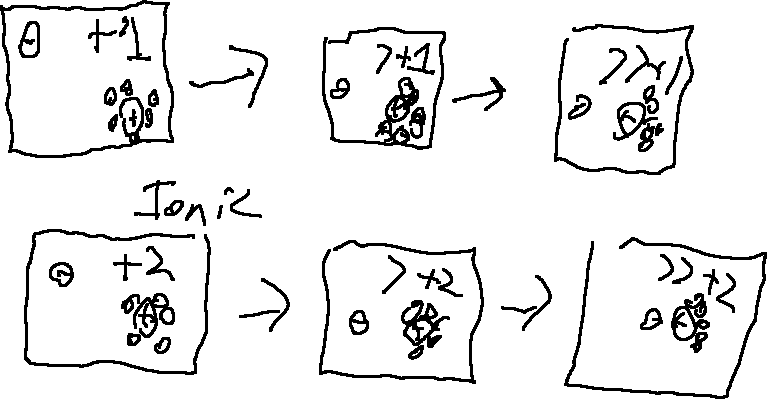
\includegraphics[width=12cm]{11-25-1.png}
	\caption*{A diagram of screening for a neutral atom and an ion}
\end{figure*}
If we look at the quadrapole transition, in order for a single photon to excite the transition we need to have the absorbed photon to have a unit of orbital angular momentum as well as spin angular momentum.

Looking at single qubit gates on an Ion we first say we can certainly use the same scheme for single qubit operations as we did for neutral atoms. If we now consider three ions in the same linear trap, these Ions should all interact with eachother via Coulomb forces.
This is because the Ions have a positive charge, so they should all repel. Clearly as we know from studying coupled harmonic oscilators, we should have several modes that our ions should be able to move in if their overall motion is excited (one mode per ion).
The lowest frequency mode should always be the center of mass motion of the ions, and then the breathing mode should be the first excited mode. If we represent our total center of mass motion with an ancilory qubit (or potentially Fock state).
We can then cause a transition at $\omega_0 + \omega_c$ (where $\omega_c$ is the frequency of the center of mass motion) which would cause a transtion from the $\ket{00}$ state (where the second qubit represents the COM state), to $\ket{11}$.
We can use all this to create a two qubit gate.
\begin{figure*}[h]
	\centering
	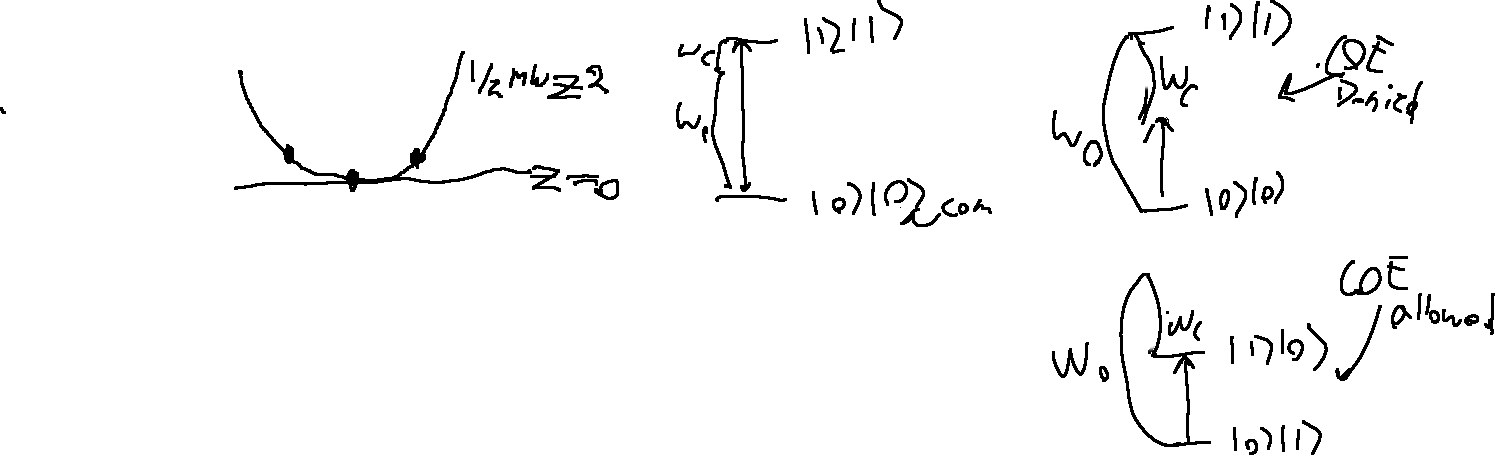
\includegraphics[width=12cm]{11-25-2.png}
	\caption*{Diagram showing the COM motion in relation to state transitions}
\end{figure*}
In order to create our controlled z gate, we first drive a $\pi$ pulse at $\omega_0 - \omega_c$ on our first qubit, then a $2\pi$ pulse on our second qubit at $\omega_0 - \omega_c$, and then finally another $\pi$ pulse on the first atom.
This all works terrifically, but it requires that our initial state has no phonons in the center of mass modes to begin with. This is a cooling process as the energy in the system will be lower after we've forced our system to have no COM phonons.
Since this process needs to be irreversible we want it to use spontaneous emission. If we repeatedly cause stimulated absorption at $\omega_0 - \omega_c$, then wait for spontaneous emission in the excited state, we can see this process will look like:
$\ket{0,n}\to\ket{1,n-1}\to\ket{0,n-1}$. Eventually we should reach a point where there are no remaining phonons, so we will be in the $\ket{1,0}$ state. In actuality we don't switch the laser on and off, and instead run it continously.
This process is known as sideband cooling.


\section*{Thanksgiving Special!!!}
We'll be doing a bit of review/Q and A today as a result of the large number of abscences for Thanksgiving.

Question: Can you go over homework 5, looking at the Schmidt decomposition/POVMs

Answer: Everything we do in quantum mechanics is about making predictions. Measurements will be described by some set of POVMs. This replaces the old system of projectors. Recall:
\begin{align*}
	\sum_n \Pi_n &= 1 &
	\Pi_n^\dagger &= \Pi_n &
	\Pi_n \geq 0
\end{align*}
Question two was of course not about prediction, but rather about retrodiction. We look at a state with classical randomness, being in either state $\ket{1}$ or $\ket{-}$.
By using a set of three POVMs rather than a standard basis of 2 measurements we can get an improvement in distinguishability between the two states.

Question: Are the set of Kraus operators the same for completely positive maps and for POVMs?

Answer: They are the same set. This can be seen because the following relations apply to Kraus operators:
\begin{align*}
	\sum_n K_n^\dagger K_n &= 1 & 
	K_n\rho K_n^\dagger \geq 0
\end{align*}
This will imply all the properties of the POVMs. Additionally of note is the fact that a POVM doesn't have a unique Kraus Operator representation, and these different representations will give different states after measurement.

Question: Problem 5, looking at the Schmidt decomposition of:
\begin{align*}
	\ket{\psi} &= \frac{\ket{00} + \ket{01} + \ket{10} - \ket{11}}{2}
\end{align*}

Answer: We want to look at the density matrix of each state seperated out, so:
\begin{align*}
	\rho_A &= \frac{1}{2}\ket{+}\bra{+} + \frac{1}{2}\ket{-}\bra{-} \\
	\rho_A &= \unit \\
	\rho_B &= \unit
\end{align*}
So this is a maximally entangled state. We pick our basis in $A$ as $\ket{+},\ket{-}$:
\begin{align*}
	\bra{+}\ket{\psi} &= \frac{1}{\sqrt{2}}\ket{0} \\
	\bra{-}\ket{\psi} &= \frac{1}{\sqrt{2}}\ket{1}
\end{align*}
So our Schmidt decomposition is then:
\begin{align*}
	\ket{\psi} &= \frac{1}{\sqrt{2}}\ket{+}\ket{0} + \frac{1}{\sqrt{2}}\ket{-}\ket{1}
\end{align*}
The size of the Schmidt decomposition can never be larger than the dimension of the smaller Hilbert space.

Question: What will the final look like?

Answer: It'll be looking at where errors happen in the quantum computers hosted by qBraid. The general idea is to run n $X$ gates to see how the error rate scales with the number of gates.
Odd and even gates may have differing behavior.


\end{document}
